\documentclass[11pt]{article}
\usepackage[margin=1in]{geometry}
\usepackage{longtable,tabularx,multirow} 
\usepackage{mathptmx, mathtools}
\usepackage{etoolbox}
\usepackage{enumitem, esvect}
\usepackage{amsmath, amsthm, amssymb}
\usepackage{float}
\usepackage{natbib}
\usepackage[hidelinks]{hyperref}
\urlstyle{same}
\bibliographystyle{apalike}
\usepackage{blindtext}
\usepackage{fontspec}
\newfontfamily\ubuntumono{Ubuntu Mono}
\usepackage{booktabs}
\setmainfont{Times New Roman}
\newcommand\tab[1][1cm]{\hspace*{#1}}
\renewcommand{\bibsection}{}
\usepackage{caption}
\usepackage{subcaption}
\usepackage{textgreek}


\title{\textbf{Processing of the Velocity Signal Extracted from Direct Numerical Simulation of a Double-Periodic Turbulent Channel Flow}}
\author{Wahyu Widhi Dyatmika - S421612}
\date{}

\begin{document}

\maketitle

\section{Introduction}
\label{sc: intro}
In this report, the data obtained from direct numerical simulation of a double-periodic turbulent channel flow is processed and analyzed in terms of physical and statistical properties. The problem definition is illustrated in Figure \ref{fig:probdef}. In the model, the surface C and D are no-slip walls, while the E-F and A-B surface pairs are assigned as periodic boundary conditions surface. The velocity components are set as \textit{u} (wall-normal), \textit{v} (span-wise), and \textit{w} (stream-wise) for the x, y, and z axes respectively. 
\begin{figure}[ht]
    \centering
    \includegraphics[width=0.5\linewidth]{Pictures/ProblemDefinition.png}
    \caption{Illustration of the problem~\citep{Józsa2023}}
    \label{fig:probdef}
\end{figure}
\\
To process the data, ParaView and MATLAB are used as the supporting software. For the ParaView, the turbulence is visualized so the coherent structures can be identified. On the other hand, MATLAB generates mean value, standard deviation, stream-wise velocity gradient, grid convergence analysis and its Richardson extrapolation, probability distribution, and correlation parameters. Furthermore, the possible experimental data collection method for future comparisons is discussed in terms of methods and variables that can be matched with the DNS results. \par
\medskip
\noindent From the result generation, all of the values are expected and in accordance with the past studies. Furthermore, particle image velocimetry (PIV) and hot wire anemometer's performance and comparable statistics to DNS results have been discussed.

\section{Methods}
\label{sc: Methods}
The data processing was conducted in ParaView and MATLAB environments. Both of the result is uploaded and updated regularly in GitHub as a means for keeping records of past developments. The details of the process of ParaView analysis and MATLAB subroutine are explained in Sections 2.1 and 2.2.

\subsection{ParaView analysis}
\label{sc: Paraview}
Using ParaView, the coherent structures of the flow are investigated. In a sense, coherent structures can be defined as a deterministic pattern or behavior of a turbulent flow \citep{Hussain1983}. This implies that in a stochastic and random behavior of a turbulent flow, an organized pattern can be extracted, and then used to understand further its elementary components and behavior regarding properties of transportation. \par
\medskip
\noindent Historically, there are various ways to identify coherent structures. One of the most popular methods is utilizing Eulerian techniques, especially Q-criterion to identify the major pattern of the flow \citep{ScK2017}. Q-criterion is defined as the areas where the vortex is higher than the rate of strain \citep{Szwabowski2021}. The Q-criterion can be expressed as 
\begin{equation}
    Q = \frac12 (||\Omega||^2 - ||S||^2)
\end{equation}
\begin{tabbing}
Where: \= \\
$||\Omega||$: \> Vorticity tensor magnitude\\
$||S||$:\> Strain rate tensor magnitude
\end{tabbing}
\noindent To generate the Q-criterion in ParaView, new vector values must initially be created. This is conducted by selecting all of the velocity components data, and then using the "AppendAttributes" option in the "Filters" tab. The new vector component is made by combining \textit{u}, \textit{v}, and \textit{w} components using the "MergeVectorComponents" feature in the "Filters" tab. After that, in the same tab, the "Gradient" feature is selected and the new vector component is selected for the scalar array. In the "Advanced Options", "Q-Criterion" is selected. Finally, the Q-criterion can be viewed using surface and surface-LIC (Line Integral Convolution) options. Additionally, the scales are adjusted so the Q-criterion is visible to evaluate.
\subsection{MATLAB Subroutine Workflow}
\label{sc: Matlab}
For the MATLAB subroutine, all of the problems will be done in one continuous subroutine. The background and algorithm process are explains in Sections 2.2.1 to 2.2.4 below.

\subsubsection{Mean Value and Standard Deviation}
\label{sc: meanvelostd}
After importing the data, the velocity arrayd is divided into their respective components. The variable names $u\_smpl$, $v\_smpl$, and $z\_smpl$ denote the sampled velocity component in the x, y, and z-axis respectively. Furthermore, the sampling location can be also obtained, designated by the variable $x\_smpl$. The mean of the sampled velocities can then be calculated using the built-in \textit{mean(f)} function, where \textit{f} is the velocity component array. The MATLAB command is based on the equation below \citep{NCL2023a}.
\begin{equation}
    \mu = \frac{1}{N} \sum^N_{i=1}{x_i}
\end{equation}
Where N is the number of data, and $x_i$ is the sampled data points which in this case are the sampled velocity components data.\\
\newline
On the other hand, standard deviation data can be obtained using \textit{std(f)} function in MATLAB, which uses calculation as the following \citep{NCL2023b}:
\begin{equation}
    \sigma = \sqrt{\frac{1}{N}\sum^N_{i=1}{(x_i-\mu)^2}}
\end{equation}


\subsubsection{Mean Stream-wise Velocity Gradient}
\label{sc: Velograd}
In this section, the mean stream-wise velocity gradient is obtained analytically and numerically. For the numerical stream-wise velocity gradient, it can be obtained by using \textit{gradient(f)} command from MATLAB. For the analytical velocity gradient, it is best to first use an existing analytical velocity equation and then differentiate said function for easier application. By viewing the mean velocity characteristics from the previous section, it is best that the analytical velocity equation uses the expression stated by von Kármán (1930) as cited in \citet[p.1]{Smart2022}
\begin{equation}
    w = \frac{w^*}{\kappa}\ln\left({\frac{x}{x_0}}\right)
\end{equation}
Where:
\begin{gather}
    w* = \sqrt{\frac{\tau_w}{\varrho}} \\
    \tau_w = 0.5c_f\rho U_b^2 \\
    c_f = \frac{0.026}{Re_b^{\frac12}}\\
    x_0 = \frac\kappa\Delta_v
\end{gather}
\begin{gather}
    \Delta_v = \frac{\nu}{w*}
\end{gather}

\noindent $U_b$ is the bulk velocity and $Re$ is the Reynolds number. The variation of the stream-wise velocity values lies in the $x$ parameters, which is the wall-normal location of the flow. Using the symbolic operations, the equations then can be derived by using \textit{gradient(f, x)} command, where \textit{x} is the sampling location array, \textit{x\_smpl}. \\
\newline
 \noindent After that, the grid convergence can be determined by varying the number of the x points. To do this, the value of \textit{x\_smpl} as the wall's normal location must be extended appropriately to the grid size. This is done by putting additional points in between every array member, and then the value of the said new points are interpolated using the two known neighboring members. After that, the new array of \textit{x\_smpl} is inputted to the analytical calculation. \\
 \newline
 \noindent Then, the errors are calculated using the $L_1$ and $L_2$ norms, which obtained from \citet{WolframL1} and \citet{WolframL2} respectively. It is worth noting that the array of the mean stream-wise velocity numerical value (\textit{w\_mean}) must be elongated to match the analytical result array by using the same procedure as the extension of the \textit{x\_smpl} so the error calculation can be conducted.
\begin{equation}
    L_1=\sum^n_i{|{w_{analytical}-w_{numerical}}|}
\end{equation}
\begin{equation}
    L_2=\sqrt{\sum^n_i{(w_{analytical}-w_{numerical})^2}}
\end{equation}
In MATLAB, the calculation of the norms is done by using \textit{norms($w_{analytical}$-$w_{numerical}$, a)} command. \textit{a} is the type of norms desired, which is 1 for $L_1$ and 2 for $L_2$. The $L_1$ and $L_2$ norms are then used for predicting the ideal error by using the Richardson extrapolation equation.

\begin{equation}
    R_{h, \frac{h}{t}}(h) = \frac{t^k \epsilon\left(\frac ht\right) - \epsilon(h)}{t^k -1}
\end{equation}

\noindent Assuming that Euler improved method is used ($k$=2) and taking the usual practice by utilizing half of the initial grid size (h/2) for the targeted smaller grid size \citep{Feldman2000}, the equation can be transformed into
\begin{equation}
    R_{h, \frac{h}{2}}(h) = \frac{4\left(\epsilon\left(\frac h2\right) - \epsilon(h)\right)}{3}
\end{equation}
In this case, the $\epsilon$ variable is the error value. The Richardson extrapolation is tested by using the grid size h, h/2, h/4, h/8, and h/16.

\subsubsection{Fast Fourier Transform}
\label{sc: fft}
In this case, the Fast Fourier Transform (FFT) method is conducted to the velocity signal at x = 0.06. Fast Fourier transform changes the signal into frequency distribution using Discrete Fourier Transform (DFT) with a faster algorithm. DFT can be expressed using the following equation \citep{Roberts2021}:
\begin{equation}
    X(k) = \sum^{N=1}_{n=0} x(t)\cdot e^{-i2\pi kn/N}
\end{equation}
\begin{tabbing}
Where: \= \\
$X(k)$: \> \textit{k}th DFT coefficient\\
$x(t)$:\> \textit{x}th sample in time-domain sequence\\
N: \> Total number of samples
\end{tabbing}

\noindent Different windowing methods are then applied to the FFT calculation. Windowing can be defined as a process to multiply the data sequence using established equations \citep{VRU2023a}. Four different windowing methods are used for the analysis, namely Hann, Hamming, Blackman, and Rectangular Window methods. \citet{Oppenheim1999} states that the Hann method changes the frequency spectra using the following equation:
\begin{equation}
    w_{Hann}(n) = 0.5 \left(1-\cos{\left(\frac{2\pi n}{N}\right)}\right)
\end{equation}
\begin{tabbing}
Where: \= \\
$w(n)$: \> \textit{n}th point window value\\
$N$:\> Number of points in the window
\end{tabbing}

\noindent Hamming method utilizes a similar algorithm as the Hann method with different values in the window function, as stated by \citet{Oppenheim1999}.
\begin{equation}
    w_{Hamming}(n) = 0.54 - 0.46\cos{\left(\frac{2\pi n}{N}\right)}
\end{equation}

On the other hand, the Blackman method utilizes two cosine functions, as shown below \citep{Wolfram2023}.
\begin{equation}
    w_{Blackman}(n) = \frac{21}{30} - \frac12 \cos({\left(\frac{2\pi n}{L-1}\right)} + \frac{2}{25}\cos{\left(\frac{4\pi n}{L-1}\right)}
\end{equation}

\noindent Lastly, the rectangular window has a fixed windowing, which is stated by \citet{Rose2011} as follows
\begin{equation}
    w_{Rectangular}(n) = 1
\end{equation}

\noindent In MATLAB, the Hann, Hamming, Blackman, and Rectangular windowing methods can be expressed using \textit{Hann(f)}, \textit{Hamming(f)}, \textit{Blackman(f)}, and \textit{Rectwin(f)} function respectively, with \textit{f} as the sampled velocity component.
\newline

\noindent The next process is employing filtering method to the FFT function. Filtering is a method to limits unwanted features from a signal \citep{VRU2023b}. There are three different methods that can be done, the first method is the moving average method, This filtering method is conducted by "averaging a number of points from the input signal to produce each point in the output signal."\citep[p.277]{Smith1998}. The method is expressed as (p.277):
\begin{equation}
    w_{Moving average} = \frac1N \sum_{j=0}^{N-1}x[i+j]
\end{equation}
In the MATLAB subroutine, this is done by using \textit{movmean(f, k)} where \textit{k} is the window length, which in this case for the sake of simplicity, is set to 5.\\
\newline
\noindent The second method used is the Gaussian filtering, the filtering equation is expressed as explained by \citet{Fatahalian2023}. In MATLAB, the filtering is conducted using \textit{timgaussfit(abs(f))} function. It is worth noting that only the real part of the FFT can be processed using this method.
\begin{equation}
    w_{Gaussian}(t) = \frac{1}{\sqrt{2\pi}\sigma}e^{-\frac{t^2}{2\sigma^2}}
\end{equation}
\newline
The last one, the Butterworth filter serves as frequency domain filtering, which filters after the time domain data is changed into frequency domain. The Butterworth filtering utilizes the following equation \citep{Butterworth1930}
\begin{equation}
    w_{Butterworth} = \frac{1}{\sqrt{1+ \left(\frac{s}{\omega_c}\right)^{2n}}}
\end{equation}
$\omega_c$ is the cutoff frequency, and $n$ is the order of the filter. In this case, the cutoff frequency is set to 0.1 Hz and the filter order is set to 4. Using the \textit{butter(filter order, cutoff frequency)} in MATLAB, value \textit{a} and \textit{b}, which are two different transfer functions can be obtained. Then using \textit{filter(b, a, f)}, the Butterworth filtering can be applied.


\subsubsection{Probability Density Distribution and Correlation Parameters}
\label{sc: Ndist}
The final process in the subroutine involves the display of the probability density function (PDF) of the velocity components and their parameters. For displaying the PDF distribution, the function \textit{[counts, edges] = histcounts(f)} is utilized, where \textit{counts} is the frequency and \textit{edges} is the range of the distribution. Then the range of the distribution is readjusted by deleting the last member of the array so the number of array members for the x and y-axis can be the same.
Then the plot can be made by using \textit{NewRange} as the X-axis and \textit{counts} as the Y-axis.\\
\newline
\noindent Then the skewness and kurtosis of the velocity components are calculated. \citet{NIST2023} states that the formula of skewness and kurtosis consequently are expressed as:
\begin{equation}
    skewness = \frac{\sum^N_{i=1}{\frac{(x_i-\mu)^3}{N}}}{\sigma^3}
\end{equation}
\begin{equation}
    kurtosis = \frac{\sum^N_{i=1}{\frac{(x_i-\mu)^4}{N}}}{\sigma^4}
\end{equation}
In MATLAB, to express both parameters one simply needs to use \textit{Skewness(f)} and \textit{kurtosis(f)}.\\
\newline
\noindent Lastly, the correlation factor between two velocity components must be determined to understand if any of the two velocity components have a statistically significant correlation. This is done by using MATLAB \textit{corrcoef(f1, f2)} function, which utilizes Pearson Correlation coefficient expressed as shown below \citep{MATLAB2023}.
\begin{equation}
    \rho(X_{i1}, X_{i2}) = \frac{1}{N-1} \sum^N_{i=1} {\frac{X_{i1}-\mu_1}{\sigma_1} \frac{X_{i2}-\mu_2}{\sigma_2}}
\end{equation}




\section{Results and Discussion}
\subsection{Paraview Analysis}
The result from ParaView post-processing is as follows. The results are viewed only at the X-Y and X-Z planes because, at the Y-Z planes, periodic boundary condition is applied thus no observed structures as there are no disturbances. 
\begin{figure}[h!]
     \centering
     \begin{subfigure}[ht]{0.49\textwidth}
         \centering
         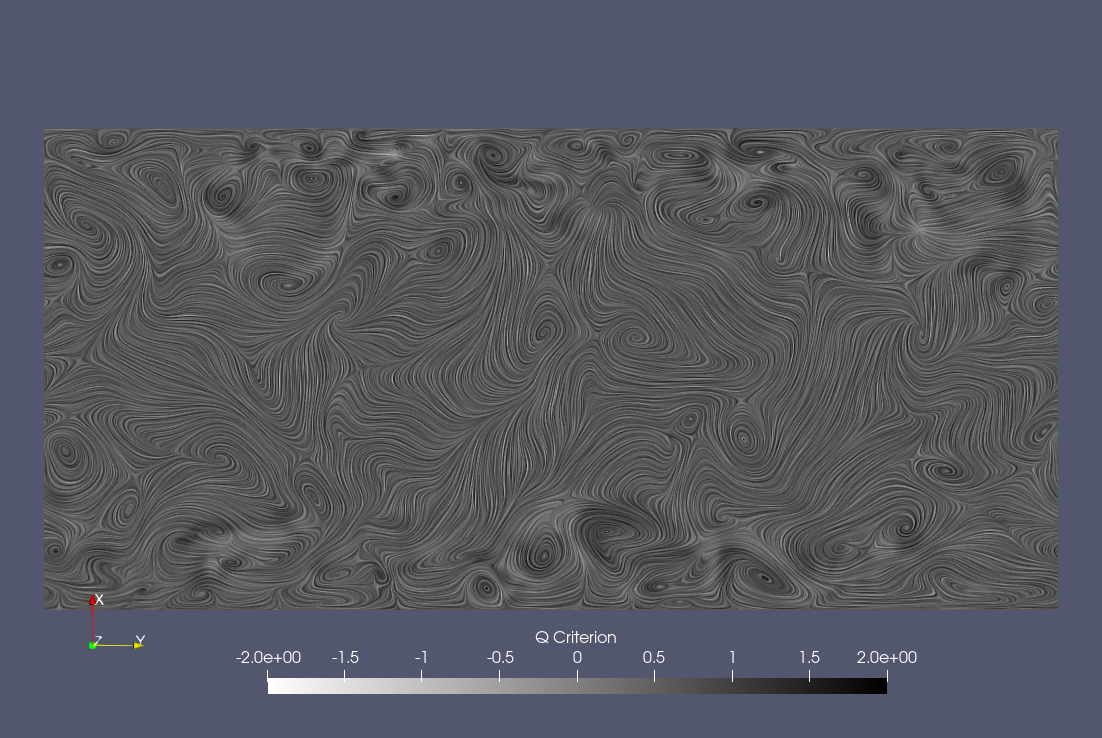
\includegraphics[width=\textwidth]{Pictures/Paraview/FrontViewLIC.png}
         \caption{Front View of LIC Surface}
         \label{fig:FVLIC}
     \end{subfigure}
     \begin{subfigure}[ht]{0.49\textwidth}
         \centering
         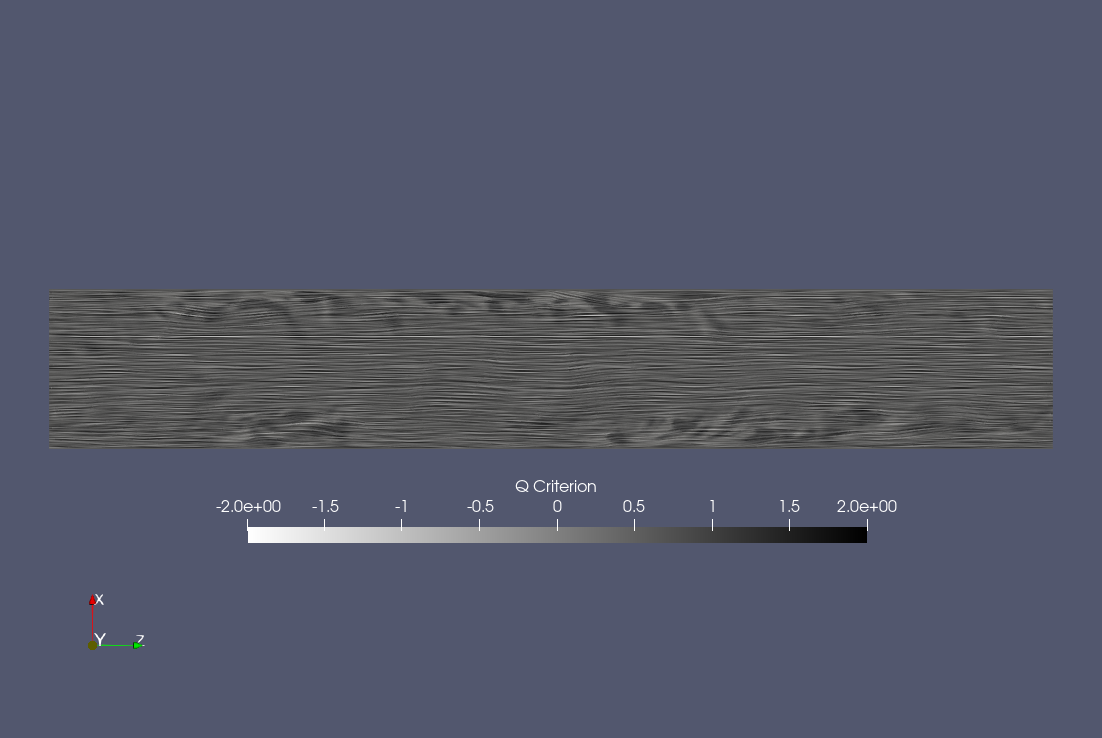
\includegraphics[width=\textwidth]{Pictures/Paraview/SideViewLIC.png}
         \caption{Side View of LIC Surface}
         \label{fig:SVLIC}
     \end{subfigure}
     \begin{subfigure}[ht]{0.49\textwidth}
         \centering
        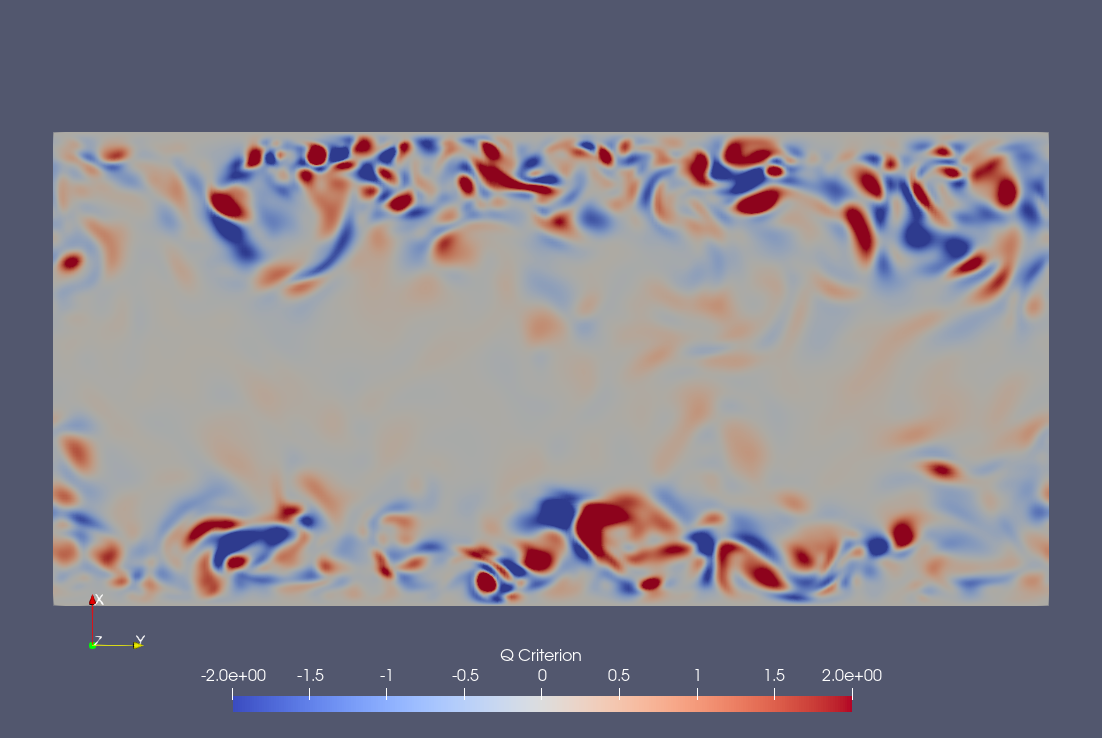
\includegraphics[width=\textwidth]{Pictures/Paraview/FrontViewSurf.png}
         \caption{Front View of Surface Contour}
         \label{fig:FVSC}
     \end{subfigure}
     \begin{subfigure}[ht]{0.49\textwidth}
         \centering
        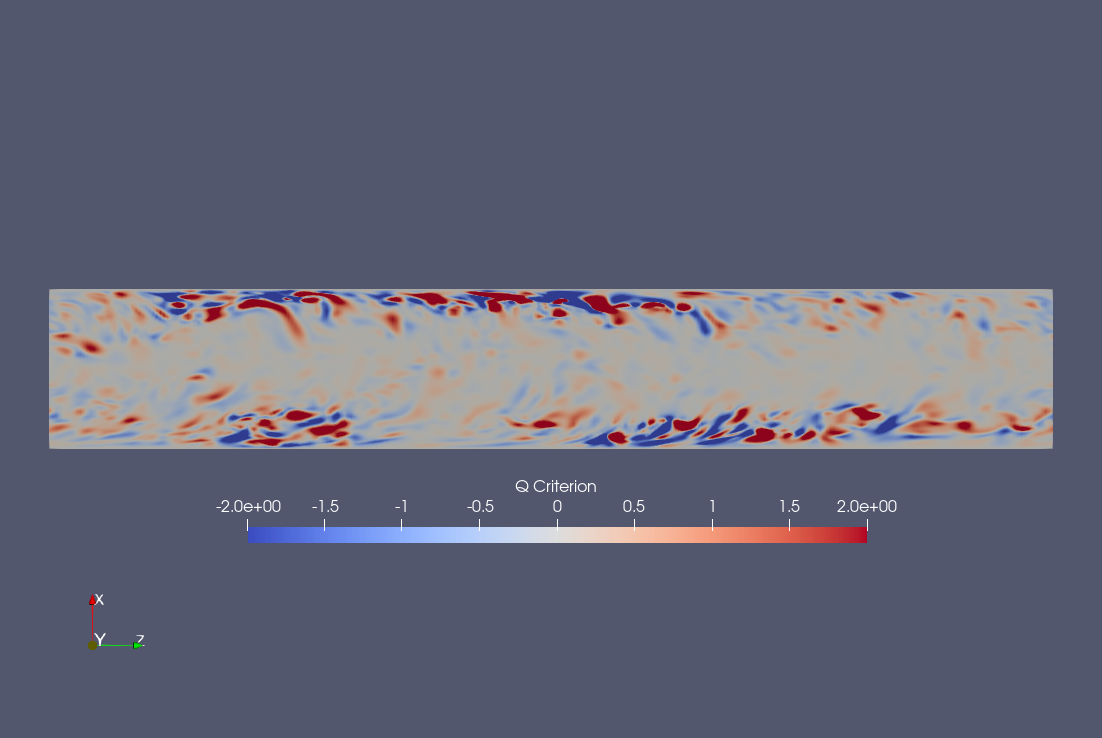
\includegraphics[width=\textwidth]{Pictures/Paraview/SideViewSurf.png}
         \caption{Side View of Surface Contour}
         \label{fig:SVSC}
     \end{subfigure}
        \caption{Coherent Structures of the Flow (ParaView Documentation)}
        \label{fig:Cohstruct}
\end{figure}
\\
\noindent As seen, there are small vortices generated near the wall as the consequences of no-slip condition. The no-slip condition states that the velocity of fluid adjacent to the wall is assumed to be the same as the velocity of the wall \citep{Day1990}. In stationary wall conditions as in this case, the value of the fluid is also zero. As a result, the velocity differences create vorticity \citep{Heijst2012}, which is observed from the surface plots.

\subsection{MATLAB Subroutine Results}
\subsubsection{Mean Value and Standard Deviation}
The resulting mean and standard deviations subroutine is displayed in the following Figure \ref{fig: MeanSTDev}. The flow visualization aligned with the flow settings mentioned in Section \ref{sc: intro}. Because the fluid flows in the z-direction, the \textit{w} velocity component is the dominant. In addition, due to a lack of flow disturbances and changes in geometric direction such as the channel bending to different directions, the \textit{u} and \textit{v} components are very close to zero value.
\begin{figure}[ht]
    \centering
    \includegraphics[width=\linewidth]{Pictures/MeanSTDev.png}
    \caption{Mean and Standard Deviation (MATLAB Documentation)}
    \label{fig: MeanSTDev}
\end{figure}
\noindent Based on the standard deviation, it can be seen that the value peaked at x = 0.0804114. This can be supported using the Law of the Wall. The peak of standard deviation is located between x+ = 5 (x = 0.0324m) and x+ = 30 (x = 0.1948m), which is the location of the buffer layer region as mentioned by Wellinger (2003) as cited by \citet{Kralik2017}. The buffer layer is characterized by highly energized turbulent flow due to instability of sheared flow \citep{Southard2023}. These instabilities can be visually recognized by the vortices generated, which shown previously in \ref{sc: Paraview}. As the consequence, flow randomness and instabilities in buffer region creates high deviation when calculated with DNS.

\subsubsection{Experimental Data Collection}
While numerical data can obtain fast and accurate data for fluid flow analysis, it is prone to unrealistic data results that do not reflect the actual fluid phenomena due to assumption and simplification. Hence, experimental data must be collected. Historically, for obtaining the velocity field components as obtained in the previous DNS calculation, there are two main experimental methods that can be used. The first is a hotwire anemometer. Hotwire anemometer works by detecting the wire cooling due to convection, which correlates with the fluid flow rate \citep{Bird1993}. Traditionally, there are three different hot wire probes --- each consisting of two wires spanning over a direction --- used to calculate the three velocity components \citep{Hodson2023}. However, there are novel methods that utilize only two probes, with two wires crossed in an X-shape \citep{ElGabry2014}. \\
\newline
\noindent The other method to acquire experimental velocity component data is Particle Image Velocimetry (PIV). PIV analysis involves seeding particles such as TiO$_2$ or oil droplets, which are let to be moved by the flow \citep{Melling1997}. Then the motion of said particles in the fluid is captured using instruments such as double pulsed laser \citep{Dantec2023}. To capture different velocity components, the capturing instruments must be placed in different directions.\\
\newline
\noindent In canonical flow analysis such as fully developed turbulent channel flow, both experimental and numerical methods result must support each other in some of the results to ensure the validity of both methods. Even though a turbulent flow can create fluctuation and uncertainty, both methods must display a good agreement in terms of low-order statistics such as mean flow and turbulence intensity \citep{Eggels1994}. In addition, high-order statistics such as skewness and flatness factors should be in agreement in both DNS and experimental methods (p.1). 

\subsubsection{Mean Stream-wise Velocity Gradient}
The result of the stream-wise mean velocity and its gradient are shown in Figure \ref{fig:VelonGrad}. As shown, the trend of the velocity and its gradient for both analytical and numerical gradient results are the same. 
\begin{figure}[ht]
    \centering
    \includegraphics[width=0.6\linewidth]{Velongrad2.png}
    \caption{Mean Stream-wise Velocity Value and Gradient}
    \label{fig:VelonGrad}
\end{figure}
\\
\noindent However, the value differs, especially in the areas near the boundary layer. This is on the basis that von Kármán analytical calculation is only accurate in the log-law layer, which is far from the boundary layer (30 $\leq$ $y^+$ $\leq$ 300), as mentioned by \citet{Arnau2023}.\\
\newline
\noindent The error can be shown in Table \ref{tab: error}. The result enforces the idea that grid convergence can be achieved, as seen with the lower error of the numerical result from the analytical result as the grid size goes lower. Additionally, using the lower grid size for Richardson extrapolation generates lower estimated ideal error.
\newpage
\begin{table}[ht]
\centering
\caption{Error for Various Grid Sizes and Richardson Extrapolation Obtained}
\label{tab: error}
\begin{tabular}{llllllllll}
\cline{2-10}
 & \textbf{$\epsilon_{h}$} & \textbf{$\epsilon_{\frac{h}{2}}$} & \textbf{$\epsilon_{\frac{h}{4}}$} & \textbf{$\epsilon_{\frac{h}{8}}$} & \textbf{$\epsilon_{\frac{h}{16}}$} & \textbf{$R_{h, \frac{h}{2}}$} & \textbf{$R_{\frac{h}{2}, \frac{h}{4}}$} & \textbf{$R_{\frac{h}{4}, \frac{h}{8}}$} & \textbf{$R_{\frac{h}{8}, \frac{h}{16}}$} \\ \hline
\textbf{$L_1$} & 5578.116 & 2799.386 & 1407.137 & 707.569 & 354.958 & 3704.972 & 1856.333 & 932.756 & 470.148 \\
\textbf{$L_2$} & 212.733 & 151.469 & 107.402 & 75.131 & 51.399 & 81.685 & 58.756 & 43.027 & 31.642 \\ \hline
\end{tabular}
\end{table}


\subsubsection{Fast Fourier Transform}
The results of FFT analysis with linear, semilog, and log-log graphs are shown in Figure \ref{fig:FFTStd}. Linear plot is difficult to analyze visually due to the high range of frequency and amplitude. Changing one or two axes into a logarithmic axis compressed the range of the graph, easing the further analysis. Due to the degree of compressing, and the availability of sources on the internet, the log-log graph is used for further FFT analysis.

\begin{figure}[ht]
    \centering
    \includegraphics[width=0.87\linewidth]{Pictures/FFTstandard.png}
    \caption{FFT Results in Linear, Semilog, and Log-Log Graph (MATLAB Documentation)}
    \label{fig:FFTStd}
\end{figure}
\noindent The results of the four windowing methods for all three velocity components are shown in Figure \ref{fig:wmethods}. 

\begin{figure}[ht]
    \centering
    \includegraphics[width=0.87\linewidth]{Pictures/Windowing.png}
    \caption{Windowing Methods Results}
    \label{fig:wmethods}
\end{figure}
\newpage
\noindent It is noteworthy to mention that the preferability of the methods is dependent on the function and  therefore must be considered based on observation \citep{NI2023}. Based on the results, it is apparent Rectangular and Hamming windows do not suppress as well as the other two methods, as the oscillations due to the Gibbs Phenomenon are massive and increased value at side lobes, which is unfavorable. Additionally, the value of spectral leakage was also observed to be present heavily in the result. Hann and Blackman methods create more side lobe attenuation and reduce oscillations. However, the Blackman method have slightly more oscillations compared to Hann, which makes Hann the most favorable windowing method. \par
\medskip
\noindent For the filtering method, the results are shown in Figure \ref{fig:filt}. The Moving Average method algorithm, while being the fastest in generating the result, has the lowest impact on the signals, as supported by \citet{Smith1998}. On the other hand, the Butterworth algorithm creates less signal distortion, as the magnitude variation in high-low frequency is lower compared to the other three. However, the amount of lag in the Butterworth filtering method is more visible than the Gaussian method. The lag is denoted by the value difference in the left side of the signal, as the signal moves to the right. While both Gaussian and Butterworth methods have their own advantages and disadvantages, Gaussian methods is the most favorable choice for the filtering method as it ensures decent frequency filtering but still minimizes lag.
\newpage
\begin{figure}[ht]
    \centering
    \includegraphics[width=0.9\linewidth]{Filtering.png}
    \caption{Results of Various Filtering Methods}
    \label{fig:filt}
\end{figure}

\noindent Additionally, the frequency spectra can be correlated with the coherent structures. In the standard channel flow, the high frequency in FFT relates to the mixing and dissipation in the flow, whereas low frequency correlates with the formation and shedding of the vortices. From the result, frequency spectra support the results in Section \ref{sc: Paraview}. The numerous amount of vortices generated corresponds with the high amplitude of low-frequency points. The mixing of the flow, while present, is not abundant in the flow. The flow condition is generally laminar (Re = 2857) which means that the turbulent condition happens only in the near wall areas.



\subsubsection{Normal Distribution and Correlation Parameters}
The result of the probability density function of the three velocity components is shown in Figure \ref{fig:PDF}. It is difficult to determine if the PDF has a normal distribution behavior with only visual judgement, therefore further quantitative judgment must be conducted.
\begin{figure}[ht]
    \centering
    \includegraphics[width=0.8\linewidth]{Pictures/PDF2.png}
    \caption{Probability Density Function of the Velocity Components}
    \label{fig:PDF}
\end{figure}
\newpage
\noindent The result of the skewness and kurtosis parameters for all of the velocity components is shown in Table \ref{tab:SkewnessKurt}. From the data, it is known that any of the velocities do not have a normal distribution, as normal distribution has zero skewness \citep{Turney2023} and has a kurtosis of 3 \citep{Zach2022}. However, for the ease of further data analysis, the distribution can be assumed to have normal distribution behavior if the distribution has kurtosis value around -7 and +7 and skewness around +2 and -2, as mentioned by Hair et al. (2010) and Bryne (2010) as cited by \citet{Watson2018}. Using the said criteria, it can be concluded that all of the velocity component distributions have normal distribution behavior.

\begin{table}[ht]
\centering
\caption{Skewness and Kurtosis Result}
\label{tab:SkewnessKurt}
\begin{tabular}{@{}llll@{}}
\toprule
 & \multicolumn{3}{c}{\textbf{Velocity Component}} \\
 & \multicolumn{1}{c}{\textit{u}} & \multicolumn{1}{c}{\textit{v}} & \multicolumn{1}{c}{\textit{w}} \\ \midrule
\textbf{Skewness} & 0.2336 & -0.0045 & -0.06988 \\
\textbf{Kurtosis} & 5.2884 & 4.2443 & 2.1419 \\ \bottomrule
\end{tabular}
\end{table}
\noindent From the command window, the correlation between two different velocity components is shown.\\
\newline
{\ubuntumono Correlation between u$\_$smpl and v$\_$smpl: -0.0017  \\  
Correlation between u$\_$smpl and w$\_$smpl: -0.1093 \\
Correlation between v$\_$smpl and w$\_$smpl:   0.0081\\}
\newline Based on the results, all of the values are near zero. Near zero, as \citet{BMJ2023} mentioned, indicates no correlation between the two variables. Therefore, it can be concluded that there is no correlation between any of the velocity components to the other.

\section{Conclusion}
All of the results have been generated successfully. The no-slip boundary condition creates a velocity difference, generating observed vortical structures near the wall. The structure has been in accordance with the past study, proving its validity.\par
\medskip
\noindent In addition, the wall-normal velocity is almost entirely dominated by \textit{w}velocity, which is the stream-wise velocity. A high standard deviation is also observed in the buffer layer region, which is expected to have highly energized turbulent flow. \par
\medskip
\noindent For the experimental data collection, the most probable methods for finding accurate data for fluid flow are PIV and hot wire anemometer. The two methods offer detailed fluid flow parameters, especially low and high-order statistics.\par
\medskip
\noindent Furthermore, stream-wise velocity gradient has been generated numerically and analytically. Even though it differs in terms of value, especially due to the analytical prediction of near-wall velocity, the difference gets lower as the number of grids increases. This confirms the grid convergence of the result. Richardson extrapolation is also proven to decrease the error between the two methods. \par
\medskip
\noindent Fast Fourier transform has been conducted to generate the frequency spectra. Four different windowing methods have been generated to multiply the signal to preferable ranges. Hann method is the most favorable windowing method. Additionally, three filtering methods as a means to allow certain frequencies have been generated. For the filtering methods, Gaussian filtering is chosen. \par
\medskip
\noindent Probability density function has been generated for all velocity components. Using visual observation, as well as skewness and kurtosis parameters, it can be proven that all of the graphs can be considered to be a normal distribution. Moreover, using correlation parameters, there is no correlation between any of the velocity components to the other.
\section{References}
\bibliography{bibliography}{}
\end{document}
